\documentclass{article}
\usepackage[utf8]{inputenc}
\usepackage{hyperref}
\usepackage{graphicx}
\usepackage{fixltx2e}
\usepackage{bm}
\setlength{\parskip}{0em}
\usepackage[margin=1.0in]{geometry}
\usepackage{pgfplots}
\usepackage{subfig}
\usepackage{url}
\usepackage{amsmath}
\usepackage[
    backend=bibtex, 
    natbib=true,
    style=numeric,
    sorting=none
    ]{biblatex}
\addbibresource{ref.bib}
\setcounter{biburllcpenalty}{7000} % required to prevent long URLs from exceeding the page margin
\setcounter{biburlucpenalty}{8000}
\pgfplotsset{width=10cm,compat=1.9}
\usepgfplotslibrary{external}
\tikzexternalize

\title{Final Project: Embedded-NIST\\
  \large ECSE 421: Embedded Systems \\ Department of Electrical and Computer Engineering \\ McGill University \\ Version 1.0}
\author{Adam Cavatassi and Jeremy Cooperstock}
\date{Winter 2018}

\begin{document}

\maketitle

\section{Introduction}
You have previously been provided with the data set that was used to train Position-NET. For your project, you will design your own neural network for an entirely new task, recognizing handwritten digits using the myRIO board. Specifically, you will "draw" numbers in the air, and use the on-board myRIO accelerometer as a sensor. How you use the data harvested by the myRIO will be up to you. Using your designed network, you must build an inference engine that will accept a new input in the form of a hand-drawn number in the air, and output its guess ("prediction") as to which number was drawn. 

%This document will guide you through the new problem definition. 

\section{Embedded-NIST}

Embedded-NIST is inspired by the MNIST dataset~\cite{mnist}, often used as the basis for simple neural network exercises.
MNIST is a dataset of thousands of small $28 \times 28$ grayscale images of hand-written digits ranging from 0 to 9. When the images are flattened to an input vector of length 784, a vanilla neural network can be easily built to recognize which of the 10 classes to which the input image belongs. 

\subsection{Data Collection}

You are required to collect data, consisting of sequences of accelerometer values, and the associated digits represented by each sequence, for example, as shown in Figure~\ref{fig:pos}.  You will then use these labelled data to train and test your neural network. Designing the training set involves determining any data processing you might want to perform, deciding how many training examples should be used for each class, and the mapping from raw accelerometer data to the input vector for your network. 

\begin{figure}[h]
\centering
\hspace{-0cm}  

\subfloat[]{{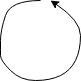
\includegraphics[scale=0.9]{figs/draw_0.png} }}%
\qquad
\subfloat[]{{
\includegraphics[scale=1.0]{figs/draw_1.png} }}%
\qquad
\subfloat[]{{
\includegraphics[scale=0.92]{figs/draw_2.png} }}%
\qquad
\subfloat[]{{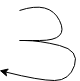
\includegraphics[scale=1]{figs/draw_3.png} }}%
\qquad
\subfloat[]{{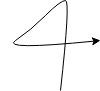
\includegraphics[scale=0.9]{figs/draw_4.png} }}%

\subfloat[]{{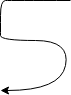
\includegraphics[scale=0.9]{figs/draw_5.png} }}%
\qquad
\subfloat[]{{
\includegraphics[scale=1.2]{figs/draw_6.png} }}%
\qquad
\subfloat[]{{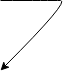
\includegraphics[scale=1.15]{figs/draw_7.png} }}%
\qquad
\subfloat[]{{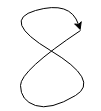
\includegraphics[scale=0.9]{figs/draw_8.png} }}%
\qquad
\subfloat[]{{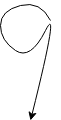
\includegraphics[scale=0.8]{figs/draw_9.png} }}%

\caption{Examples of hand-drawn numbers on a 2-dimensional plane.}

\label{fig:pos}
\end{figure}

\subsection{Network Design}

You are free to choose the parameters that govern the design of the neural network for this project, i.e., the size of the input/output vectors, the number and size of the hidden layers, the loss function, learning rate, and activation function.
Optimizing a neural network can be time-consuming, and a modular implementation, which you have hopefully achieved through the previous labs in this course, will likely help speed up your design process, allowing you to investigate the effectiveness of various network configurations more quickly. 


\subsection{External Code}

For file manipulation and data shaping needed to build your training set, e.g., to clean or trim your raw data, you are permitted to use an external software environment such as MATLAB, Python, or Excel. However, any operations required for the real-time inference engine must be performed entierly within LabVIEW. For example, assuming you have a trained network, you are {\em not} allowed to input a new data sample e.g., drawing a 3, then stop your LabVIEW code, carry out some computation with Python, and use those results to resume your LabVIEW code.

\section{Submission requirements}

Much like in previous labs, you must submit a .zip file containing your project file, all VI files that are part of your project, and screenshots of both the final block diagram and final front panel for all VIs. You must also submit the code used for any scripts used to manipulate training data. The front panel of your training VI should include a plot of training and validation set errors over time, as well as a data collection interface. You will also be required to submit a URL to a private YouTube video with a maximum length of 300 seconds that demonstrates the full functionality of the network training, including an error plot followed by the inference engine that you trained in real-time.

Your group will be required to demonstrate the performance of your system, live, in class, during the final week of the semester.  Sign up for the presentation slots will be made available shortly.

If you saved a set of weights that perform well, you may use those to demonstrate the inference engine.  However, you must {\em also} demonstrate that your system is able to learn the weights, as was stipulated for Lab 4. %This concession is being made because the random nature to the weight initialization means that you may not always obtain a good training result every time you run your code.
You should demonstrate the best possible inference engine you are able to achieve, convincing the viewer that your your weights were synthesized from your code and your own data. Your network outputs can be determined by you, as long as they are very clear. 

Show that each hand-drawn digit is clearly recognized by the neural network after training. You are also required to submit a formal report in the IEEE conference format. The report should outline the methodology used to build your data set and neural network, and should disclose all design parameters explored as well as results from the project such as training loss and computation time. The report should evaluate the effectiveness of your approach.


\printbibliography

\onecolumn

\end{document}
